\subsection{BIG-Bench (Beyond the Imitation Game Benchmark)}
{{\footnotesize
\noindent BIG-Bench is a collaborative suite of 204 tasks designed to probe LLMs' reasoning, 
knowledge, and bias across diverse domains and difficulty levels beyond simple imitation.


\begin{description}[labelwidth=4cm, labelsep=1em, leftmargin=4cm, itemsep=0.1em, parsep=0em]
  \item[date:] 2022-06-09
  \item[version:] 1
  \item[last\_updated:] 2022-06-09
  \item[expired:] false
  \item[valid:] yes
  \item[valid\_date:] 2022-06-09
  \item[url:] \href{https://github.com/google/BIG-bench}{https://github.com/google/BIG-bench}
  \item[doi:] 10.48550/arXiv.2206.04615
  \item[domain:] NLP; AI Evaluation
  \item[focus:] Diverse reasoning and generalization tasks
  \item[keywords:]
    - few-shot
    - multi-task
    - bias analysis
  \item[licensing:] Apache-2.0
  \item[task\_types:]
    - Few-shot evaluation
    - Multi-task evaluation
  \item[ai\_capability\_measured:]
    - Reasoning and generalization across diverse tasks
  \item[metrics:]
    - Accuracy
    - Task-specific metrics
  \item[models:]
    - GPT-3
    - Dense Transformers
    - Sparse Transformers
  \item[ml\_motif:]
    - LLM evaluation
  \item[type:] Benchmark
  \item[ml\_task:]
    - Supervised Learning
  \item[solutions:] Multiple, including human baselines
  \item[notes:] Human baselines included
  \item[contact.name:] Aarohi Srivastava et al.
  \item[contact.email:] bigbench@googlegroups.com
  \item[datasets.links.name:] BIG-Bench GitHub Repository (contains tasks and data)
  \item[datasets.links.url:] \href{https://github.com/google/BIG-bench/tree/main/bigbench/benchmark\_tasks}{https://github.com/google/BIG-bench/tree/main/bigbench/benchmark\_tasks}
  \item[results.links.name:] BIG-Bench GitHub Repository (results in papers and code)
  \item[results.links.url:] \href{https://github.com/google/BIG-bench}{https://github.com/google/BIG-bench}
  \item[fair.reproducible:] True
  \item[fair.benchmark\_ready:] True
  \item[id:] big-bench\_beyond\_the\_imitation\_game\_benchmark
  \item[Citations:] \cite{srivastava2023imitationgamequantifyingextrapolating}
\end{description}

{\bf Ratings:} ~ \\

\begin{tabular}{p{0.15\textwidth} p{0.07\textwidth} p{0.7\textwidth}}
\hline
Rating & Value & Reason \\
\hline
dataset & 5 & Public, versioned, and well-documented; FAIR overall
 \\
documentation & 5 & Explained in the associated paper.
 \\
metrics & 5 & Many tasks use standard quantitative metrics (accuracy, BLEU, F1). Others involve subjective ratings (e.g., Likert), which reduces cross-task comparability.
 \\
reference\_solution & 2 & Human baselines and LLM performance results are included; however, runnable reference solutions are limited and setup is not fully turnkey.
 \\
software & 4.5 & Quick start notebook provided, but instructions on how to run it are lacking.
 \\
specification & 4.5 & Tasks are diverse and clearly described; input/output formats are usually defined but vary widely, and system constraints are not standardized.
 \\
\hline
\end{tabular}

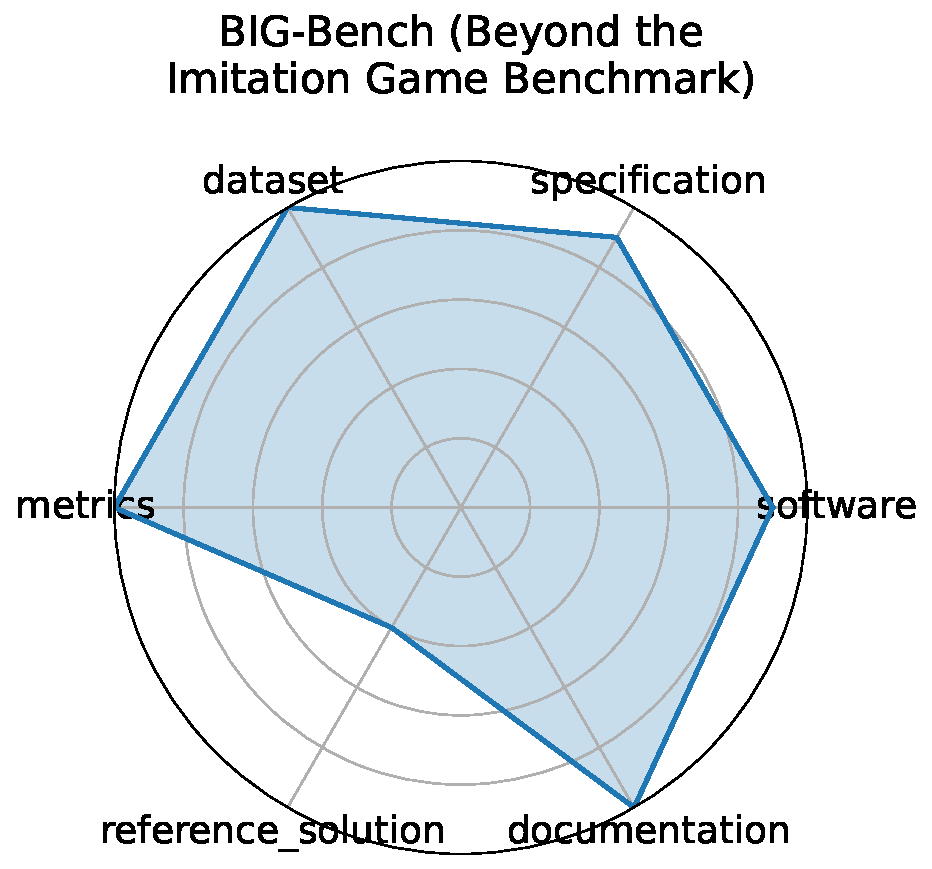
\includegraphics[width=0.2\textwidth]{big-bench_beyond_the_imitation_game_benchmark_radar.pdf}
}}
\clearpage